\subsection{Concepts for Data Preparation and Modeling}

In this section, concepts and processes, which are applied during
data preparation and modeling, are discussed theoretically.
The practical implementation is shown in sections \ref{sec:Data Preparation} and \ref{sec:Modeling}.

\subsubsection{Mean Removal, Variance Scaling and Standardization}
\label{sec:Mean Removal, Variance Scaling and Standardization}
During the data preparation stage of model development, it can be helpful to transform the data into a different shape
to improve the results of a model \cite[35]{Subasi2020}. This subsection explains some methods of data transformation, which are used in the
implementation section.

\textbf{Mean Removal} is the process of shifting the data in a column, so that the mean $\overline{x}$ of all datapoints in the
column is equal to $0$ \cite{ScikitPreprocessing}.
An example set of integers $a_1 = \{6, 7, 2, 1\}$ has a mean of $\overline{x_1} = 4$.
Removing it's mean without distorting other properties of the data entails subtracting $4$ from each member of the
set, resulting in a new set $a_2 = \{2, 3, -2, -3\}$ with $\overline{x_2} = 0$. The dataset is now centered around $0$.

\textbf{Variance Scaling} involves transforming the data in a way, that each column has unit variance, meaning variance
$\sigma^2 = 1$ \cite{ScikitPreprocessing}. This is done by dividing each member of the column by the column's standard deviation.
An example set of integers $b_1 = \{6, 7, 2, 1\}$ has standard deviation $\sigma_1 = 2.94$ and variance $\sigma_1^2 = 8.67$.
Dividing each member of $b_1$ by $\sigma_1$ results in the set $b_2 = \{2.04, 2.38, 0.68, 0.34\}$ with variance $\sigma_2^2 = 1$.

\textbf{Standardization} involves performing both mean removal and variance scaling on a column \cite{ScikitPreprocessing}.
Standardizing an example set $c_1 = \{6, 7, 2, 1\}$ would result in the following set $c_2 = \{0.68, 1.02, -0.68, 01.02\}$.
Standardized features are normally distributed. Many Machine Learning Algorithms have improved results when receiving standardized input
data. It has the additional benefit of equalizing the impact of features while keeping valuable information about the outliers
and value range \cite[35]{Subasi2020}.

\subsubsection{Dimension Reduction}
\label{sec:Dimension Reduction}

Dimension reduction refers to reducing the number of dimensions
in the input data, while keeping the highest possible amount of information from
the original dataset \cite[53]{Subasi2020}. The benefit of this is that some features might not contribute to a better model,
but instead promote bias and overfitting.
There are multiple ways to reduce dimensions, such as feature selection, where some features, which don't
contribute to a better model, are simply removed \cite[55]{Subasi2020}.
New features can be constructed by using data from different original features and
combining it into one, also reducing dimensionality.
Another approach is \ac{PCA}. Here, features are constructed by finding
principal components in a dataset \cite[62f]{Subasi2020}. This is done by projecting the data into m-dimensional space,
where each feature is contained in one spatial dimension.
The first principal component is found by rotating the feature space to find the direction
which offers the highest variance in the whole dataset.
The second component must be orthogonal to the first one and again have the highest variance
of all possible directions. This can be repeated to create as many principal components as are benefitial to the model \cite[62f]{Subasi2020}.
Dimension reduction using \ac{PCA} was attempted as part of this project,
but is not explained deeper as it didn't yield great result for the dataset.

\subsubsection{Hyperparameter Optimization}

Machine learning models have two types of parameters: model parameters and hyperparameters.
Model parameters are values, which are optimized using training data during the training process.
They are not specified in advance \cite[21]{Raschka2018}.
Hyperparameters, on the other hand, are not optimized using data, but are specified before training.
They are like "settings" for the estimator \cite{scikit-hyperparameters}.

Even though hyperparameters are not optimized during training,
there are multiple ways to find the best set of hyperparameters.
In this project, grid search is used, which takes a parameter grid containing
multiple values for each hyperparameter as input \cite{scikit-hyperparameters}.
A model is trained using every possible combination of all given values on the grid and a score
is calculated for each model. The best combination of hyperparameters are the ones used on the model
with the highest score. This might not be the optimal set of hyperparameters though, as only values
in the search grid are considered.

\subsubsection{K-fold Cross Validation}

When training a model, it is necessary to split the data into train and test samples.
Using the same data for training and calculating the accuracy
score of a model would result in a model, that is fitted exactly to the training
data. It will perform very well on that data, but will fail to make predictions on any data
it has not yet seen. This is called overfitting \cite[7]{Raschka2018}.

When optimizing the hyperparameters of an estimator, one could use the test set to score
the model and find the best parameters. A problem with this approach is, that now test data,
which should be completely independent from the training process,
is involved in the optimization process, which could lead to the hyperparameters being
"fitted" to the test data \cite{scikit-cross-validation}.

\ac{CV} is a solution to this problem. During optimization, the training set is
split into $k$ groups, named folds. A given estimator is trained on $k-1$ folds and its accuracy
is calculated using the samples in the remaining folds. This is done $k$ times, using a different fold
for scoring each time. The average of all scores is the cross-validation score, giving a good
representation of the overall performance of the estimator.
The benefit of this is, that test data is kept completely seperate from training data, but there
is still a good way of evaluating the performance of an estimator trained with a given set
of hyperparameters. This is crucial during hyperparameter optimization, as the best parameters
can not be found without a good way to score each model \cite[24f]{Raschka2018} \cite{scikit-cross-validation}.
Figure \ref{fig:cross validation workflow} shows a typical workflow when using cross validation
and hyperparameter tuning to create a model. Figure \ref{fig:cv data segmentation} shows,
how the data is segmented when using 5-fold cross validation on the training set.

\begin{figure}[H]
    \centering
    \caption{Typical Cross Validation Workflow}
	\label{fig:cross validation workflow}
    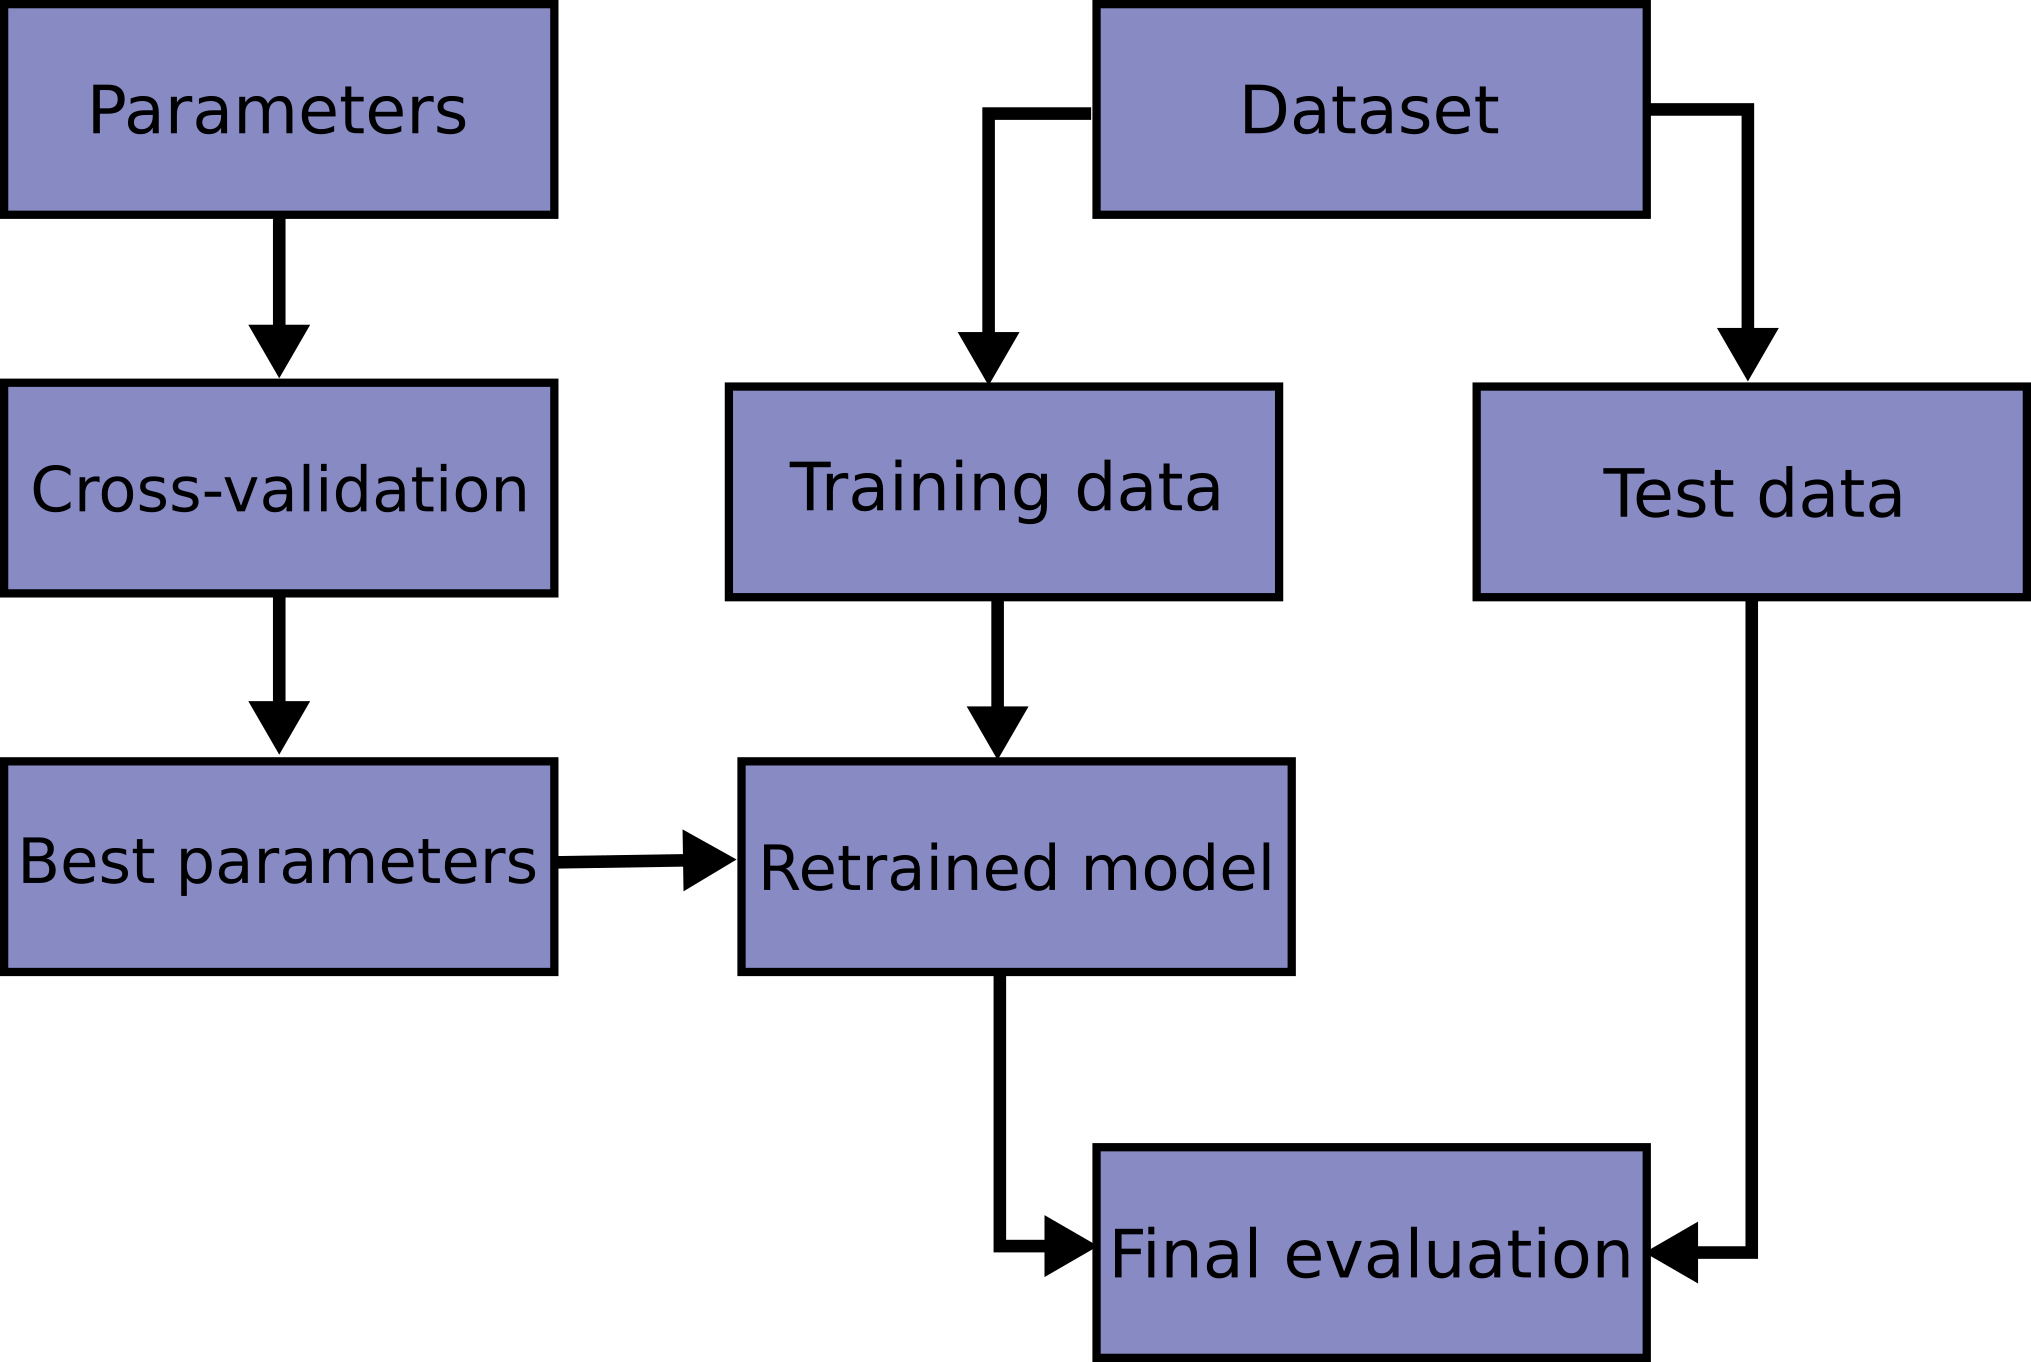
\includegraphics[width=0.6\textwidth]{cv_workflow}
    \\
    Source: \cite{scikit-cross-validation}
\end{figure}

\begin{figure}[H]
    \centering
    \caption{Data Segmentation for Cross Validation}
	\label{fig:cv data segmentation}
    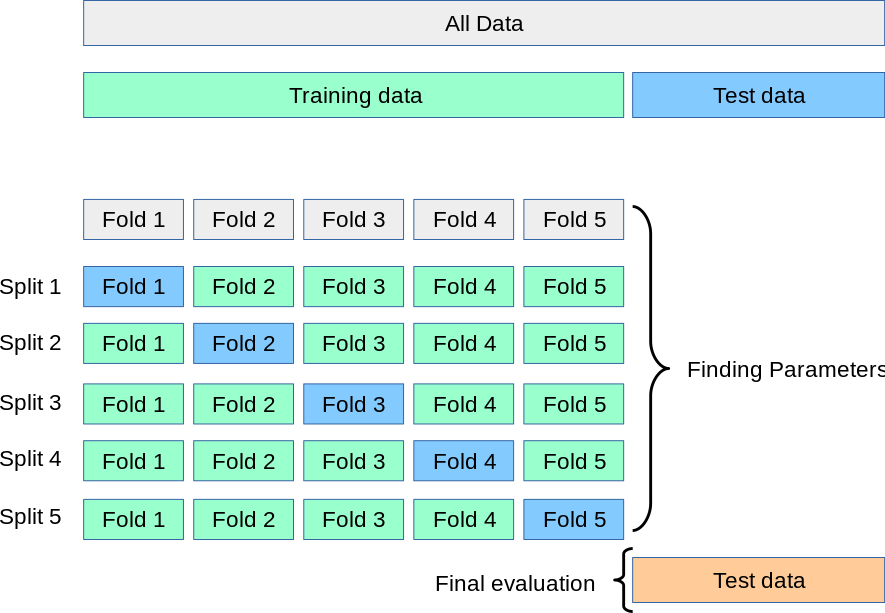
\includegraphics[width=0.6\textwidth]{cv_data_segmentation}
    \\
    Source: \cite{scikit-cross-validation}
\end{figure}